\documentclass[10pt, letterpaper]{article}
%\usepackage[cm]{fullpage}
\usepackage{algpseudocode}
\usepackage{algorithm}
\usepackage{graphicx}
\usepackage[section]{placeins}
\usepackage[table]{xcolor}
\usepackage{amsmath}
\usepackage[margin=0.5in]{geometry}


\algrenewcommand\Return{\State \algorithmicreturn{} }%


\title{Largest Subarray}
\author{Daiwei Chen \and Joseph Watts}

\begin{document}
	\maketitle
	\begin{abstract}
		Calculating the maximum sum of values within a contiguous subset of an array is a problem mostly found in the field of image processing.
		This paper explores the impact of using two different approaches to solve this problem when one approach is using a brute force algorithm, and the other is using Kadane's algorithm, a well known, more optimized approach.
		Due to the different complexity of the two algorithms used to solve this problem,
		there will be a noticeable performance impact when comparing the time taken to run over arrays of different lengths. 
	\end{abstract}
	\section{Background and Related Work}
  Finding the largest subarray is a problem that has to deal with finding a contiguous subarray within a given list, $L$, where the found subarray has a sum higher than any other possible subarrays within $L$.
  This algorithm is important to its real world use cases. One such use as computer vision, to find the brightest area within an image, it's basically a ``Maximum Subarray'' problem on the lumens within the list of pixels.

	\subsection{Brute Force Algorithm}

	\begin{algorithm}
	\begin{algorithmic}
		\caption{Brute Force}\label{bruteforce}
	\Function{bruteForce}{A}
	\State $n\gets len(A)$
	\State $maxsum\gets A[0]$
	\For{$i$ in 0..$n$-1}
	\For{$j$ in $i$..$n$-1}
	\State $total\gets 0$
	\For{$k$ in $i$..$j$}
	\State $total\gets total + A[k]$
	\EndFor
	\If{$maxsum < total$}
	\State $maxsum\gets total$
	\EndIf
	\EndFor
	\EndFor
	\EndFunction
	\end{algorithmic}
	\end{algorithm}


	This brute force algorithm works by keeping track of both a start and ending index, and then calculating a sum for all the indexes between.
	The starting index goes from the position of the first element until the last element, while the ending index repeats for all values between the starting index and the position of the last element.
	A third loop then sums all the values found between these two indexes.
	% Summation Equation
	\[\sum_{i = 0}^{n-1}\sum_{j = i}^{n-1}\sum_{k = i}^{j}1\]

	The outer loop keeps track of $i$, the starting index, and runs the entire length of the array, or $n$ times.
	The middle loop keeps track $j$, the ending index, and runs the length between $i$ and the end of the array, $n$.
	There is then another inner value, $k$, which runs between the values of $i$ and $j$.

	Due to these three nested summations, this brute force algorithm will run in $O(n^3)$ time.

	\subsection{Kadane Algorithm}

  \begin{algorithm}
		\caption{Kadane Algorithm}\label{kadane}
	\begin{algorithmic}
	  \Function{Kadane}{L}
    \State $maxEnding \gets L[0]$
    \State $maxAlways \gets L[0]$
    \For{i 1..len(L)}
    \State $maxEnding \gets \Call{max}{L[i], maxEnding + L[i]}$
    \State $maxAlways \gets \Call{max}{maxAlways, maxEnding}$
    \EndFor
	  \Return{$maxAlways$}
	  \EndFunction
	\end{algorithmic}
	\end{algorithm}
  Kadane is a very good example of a simple but effective way to show the benefits of using dynamic programming.
  This algorithm works by keeping track of variables, $maxEnding$ and $maxAlways$.
  $maxAlways$ holds the value of the current largest sum.
  $maxEnding$ holds the value of the largest subset, but only within the current iteration of $i$. 
  Because it keeps track of what sums have been calculated, it does not have to recalculate these same subarrays during the next iteration.
  This will remove two nested for loops which are present within the brute force algorithm.

  \[
  \sum_1^n2 \\
  = 2 * n \\
  = \Theta(n)
		\]
	This algorithm is $\Theta(n)$ because it only iterates through each element of the array once.
	\section{Experimental Setup}
	For the experimental setup, we have allowed our users to either input an array to test both algorithms against, or run our own tests.
  Our own tests included of multiple n values that will be timed. For each n value, we randomly generate n numbers of numbers between -5 and 5 inclusive and place them into a list. We then will time each run of the Brute Force algorithm and Kadane algorithm to go through that list of random numbers. After about 100 trials for each n, we will collecte all the timing data and proceed to find the averge run time for both algorithms for that n.
  Timing data is collected by using a high definition clock within Rust. These timings were done on an Intel Xenon X5570 processor clocked at 2.9GHz. The host machine was running a 64bit version of Fedora 29 Server Edition.
	\section{Results}

Below are the results found by running both the brute force algorithm and Kadane's algorithm against varying lengths of arrays ranging from a length of 1 to 3500.

	\begin{figure}[htbp]
		\begin{center}
			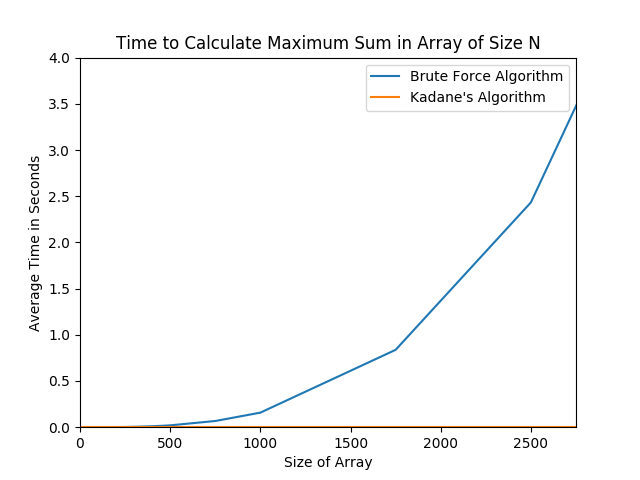
\includegraphics[width=0.70\textwidth]{python/avgTimeGraph.png}
			\caption{Time to Calculate Maximum Sum in Array of Length $n$}
			\label{fig:time-graph}
		\end{center}
	\end{figure}


\begin{table}[htb!]
	\begin{center}
	\caption{
		\label{fig:time-table} Table of Brute Force vs Kadane Timings}
	\medskip
	\begin{tabular}{ | p{2cm} | l | l | }
		\hline
		Size of Array & Brute Force (s) & Kadane (s) \\ \hline
		1 & 0.000000033 & 0.000000025 \\ \hline
		5 & 0.000000085 & 0.000000036 \\ \hline
		10 & 0.000000448 & 0.000000051 \\ \hline
		50 & 0.000030930 & 0.000000125 \\ \hline
		100 & 0.000194367 & 0.000000184 \\ \hline
		150 & 0.000594095 & 0.000000260 \\ \hline
		200 & 0.001366055 & 0.000000331 \\ \hline
		250 & 0.002607847 & 0.000000402 \\ \hline
		300 & 0.004420136 & 0.000000466 \\ \hline
		350 & 0.006950275 & 0.000000573 \\ \hline
		400 & 0.010421218 & 0.000000639 \\ \hline
		450 & 0.014655456 & 0.000000716 \\ \hline
		500 & 0.020030729 & 0.000000956 \\ \hline
		750 & 0.067125954 & 0.000001231 \\ \hline
		1000 & 0.157617270 & 0.000001779 \\ \hline
		1750 & 0.837418008 & 0.000002682 \\ \hline
		2500 & 2.432867191 & 0.000003601 \\ \hline
		3500 & 6.606255604 & 0.000005064 \\ \hline
	\end{tabular}
	\end{center}
\end{table}

	\section{Conclusions}
	As cleary shown through our graph and time table found in Section 3,
	Kadane's algorithm is a much more optimized solution to solve the problem of finding the maximum sum of values within an array.
	The brute force implementation previously described runs in $O(n^3).$
	At the same time Kadane's algorithm runs in $O(n)$ time due to only looping through the elements of the array one time.
	Generally it would be much faster to use Kadane's algorithm to solve this problem.
\end{document}
